\section*{1. Setting}
The tetrad geometry Letter \cite{letter} derives the regular dual tetrahedra within its frame assumptions. The vortex proof \cite{vortex} establishes circulating states on the associated graphs. The sustained Stage VII flywheel \cite{flywheel} gives an explicit conservative solution with eight outer rings and a shared core. We ask for a reverse algebraic reconstruction, starting with only the inherited labels and norm, without inserting spatial coordinates. Let $W=\one^\perp\subset\R^4$, $J=\one\one^T$, $G=\G$ and $P=G/4$.
\begin{theorem}[Cycle Gram]
Let $B$ be the vertex-edge incidence of $K_4$, orienting the six edges from smaller to larger label, with tail $-1$ and head $+1$. Let $D$ be the $6\times4$ matrix of consistently oriented boundaries of the four complementary triangles. Then
\begin{equation}
\begin{gathered}BB^T=D^TD=G,\quad BD=0,\\D\one=0,\quad \operatorname{im}D=\ker B.\end{gathered}
\end{equation}
Moreover $DD^T/4=I_6-B^TB/4$.
\end{theorem}
\begin{proof}
Each vertex has three incident edges, and two vertices share one edge with opposite incidence. Each oriented triangle has three edges, and any two triangles share one edge traversed in opposite directions (orient the faces by the boundary of the abstract ordered simplex). This gives both Gram matrices. Boundary of boundary gives $BD=0$; the Gram gives $D\one=0$ and rank three. Connectedness of $K_4$ gives rank $B=3$, so the containment $\operatorname{im}D\subseteq\ker B$ is equality. The stated projectors follow from $G=4P$.
\end{proof}
\begin{figure*}[t]\centering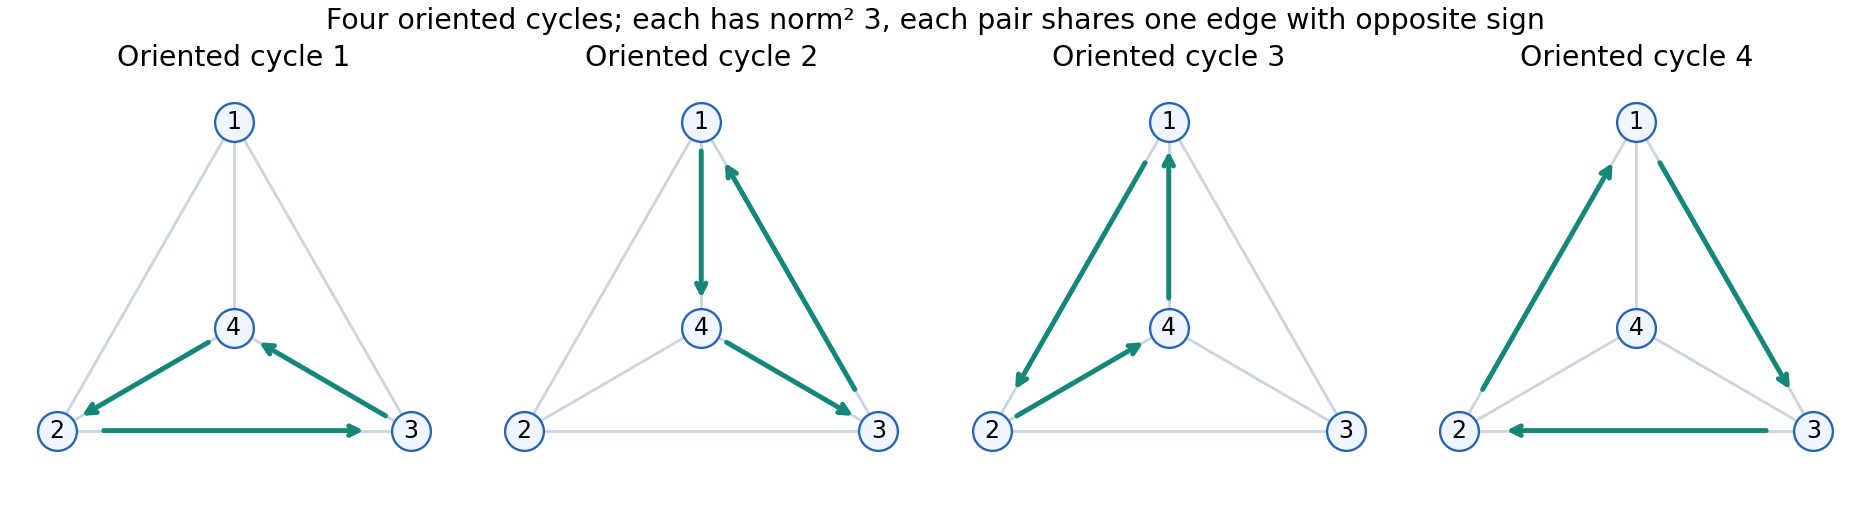
\includegraphics[width=.79\textwidth]{four_cycles.png}\caption{The four oriented cycles of the abstract four-leg graph, before spatial reconstruction.}\label{fig:cycles}\end{figure*}
\smallskip
\textbf{Metric qualification.} The cycle columns have length $\sqrt3$ and mutual cosine $-1/3$. With a positive diagonal edge metric $\operatorname{diag}(w_e)$, an off-diagonal Gram entry is minus the weight of the corresponding shared edge. Equality of all off-diagonal entries therefore holds exactly when all six weights are equal. More generally, a permutation-invariant symmetric form on $W$, extended by zero on constants, has constant diagonal and constant off-diagonal and hence is a multiple of $P$. The equal-edge norm is an inherited symmetry premise, not a dynamical consequence.
\section*{2. The independent flywheel read}
\begin{theorem}[Column Gram and minimum-norm pattern]
In one chamber label the twelve outer tiles $(i,j)$ with $i\ne j$. Let $R$ and $Q$ sum rows and columns. In the native Euclidean norm put $P_r=I_{12}-R^TR/3$, $C=QP_r$, $F=\sqrt{3/2}\,C^T$. Then
\begin{equation}
 CC^T=\tfrac23G,\qquad F^TF=G.
\end{equation}
For $q\in W\otimes\C$ the unique minimum-norm row-closed array satisfying $QX=q$ is
\begin{equation}
 \begin{gathered}X=\tfrac38 C^Tq,\quad X_{ij}=\tfrac38(q_j+q_i/3),\\
 \|X\|^2=\tfrac38\|q\|^2.\end{gathered}
\end{equation}
\end{theorem}
\begin{proof}
Each row has three entries, so $RR^T=3I$ and $P_r$ is the orthogonal projector onto $\ker R$. Each column read has three positions of projector diagonal $2/3$. Distinct columns share two rows whose off-diagonal projector entry is $-1/3$. This gives $CC^T=(8/3)P$. The stated right inverse therefore satisfies the constraints. It is orthogonal to all perturbations in $\ker R\cap\ker Q$; Pythagoras proves strict minimality. Its components follow by subtracting the mean of the three column values in each row, using $\sum q_i=0$. The squared norm follows from $CC^T$.
\end{proof}
\begin{theorem}[Oriented isometry]
The map $L=DF^T/4$ satisfies $LF=D$, $L^TL=FF^T/4$, and $LL^T=DD^T/4$. For any permutation $p$ let $T,U,V$ act on labels, ordered tiles and oriented unordered edges, respectively. Then
\begin{equation}
 UF=FT,\qquad VD=\operatorname{sgn}(p)DT,
 \qquad VL=\operatorname{sgn}(p)LU.
\end{equation}
\end{theorem}
\begin{proof}
Insert $F^TF=D^TD=4P$ and $F\one=D\one=0$. The row/column read commutes with relabeling; the oriented simplex boundary gains the permutation sign. Since the actions are orthogonal, the two covariance identities imply the last one. Thus the isometry is equivariant for proper tetrahedral rotations and sign-twisted under reflections.
\end{proof}
\begin{figure*}[t]\centering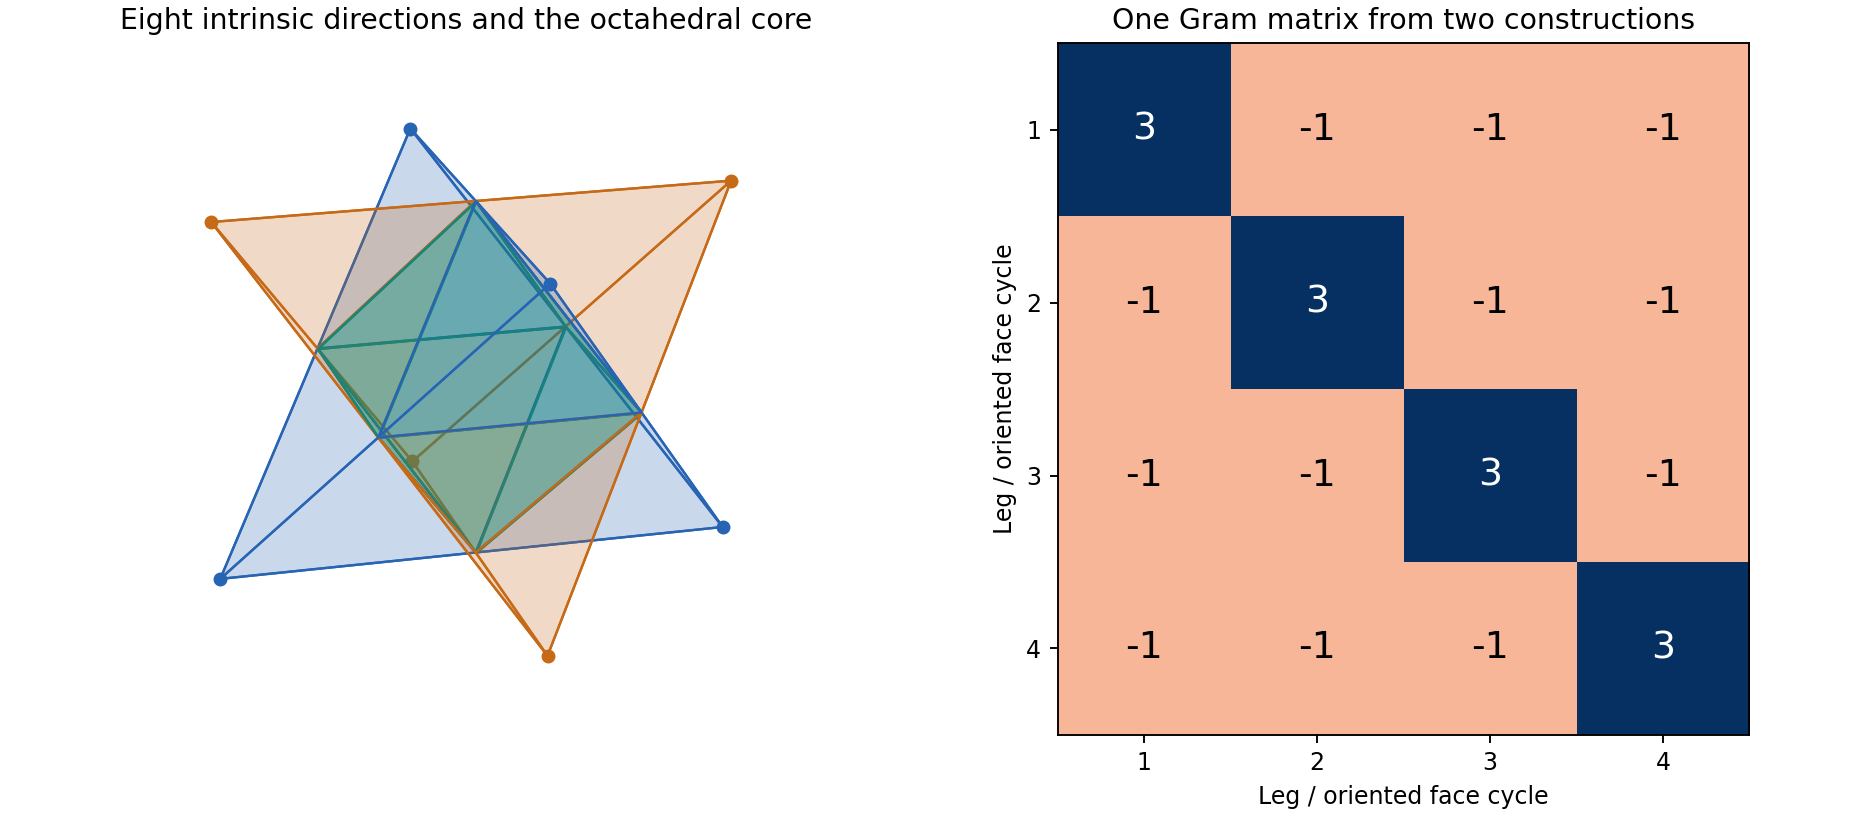
\includegraphics[width=.72\textwidth]{geometry_gram.png}\caption{The intrinsic Gram matrix and the reconstructed dual tetrahedra with their shared octahedral core.}\label{fig:geometry}\end{figure*}
\section*{3. The actual octahedral core and the current identity}
\begin{theorem}[The three-dimensional collective core]
The twelve core bonds $y_i^+\to y_j^-$, $i\ne j$, form the connected graph $K_{4,4}$ minus a matching. Its divergence-free current space has dimension five. Under chamber inversion $I\mapsto-I^T$, its even and odd sectors have dimensions three and two, respectively. The even sector is the four-leg cycle space, with each antisymmetric edge entry duplicated with opposite sign. The map divided by $\sqrt2$ is an isometry.
\end{theorem}
\begin{proof}
The $4\times4$ current array has zero diagonal. Divergence-free means zero row and column sums. The connected dual graph gives dimension $12-8+1=5$. Inversion reverses orientation and interchanges the indices. For the even sector the array is antisymmetric, with six free entries before the rank-three incidence constraints $Ba=0$. For the odd sector the array is symmetric, with six entries before four independent row constraints. Independence follows because a dependence with coefficients $c_i$ requires $c_i+c_j=0$ for every distinct pair, forcing zero by any triangle. Antisymmetric duplication doubles squared norm.
\end{proof}
\begin{theorem}[Collective phase and edge current]
For the existing collective phase $q=x+iy\in W\otimes\C$, define $a_{ij}=\operatorname{Im}(\bar q_iq_j)=x_i y_j-y_i x_j$ for $i<j$. Then
\begin{equation}
 Ba=0,\quad j_0=D^Ta,\quad Dj_0=4a.
\end{equation}
Every direction of the even core cycle space is realized by such a phase wedge. For the published Stage VII amplitudes $X_{ij}^{\pm}=\rho(uq_i+vq_j)$ and $y_i^{\pm}=\rho wq_i$, with ring and central hoppings $r=k=-1$, the oriented mean ring currents $j$ of the positive stellations and the six core entries $I_{<}$ satisfy
\begin{equation}
 \begin{gathered}j=\frac{2\rho^2|v|^2}{3}D^Ta,\quad I_{<}=2\rho^2|w|^2 a,\\
 \boxed{|v|^2 I_{<}=\tfrac34 |w|^2 Dj.}\end{gathered}
\end{equation}
\end{theorem}
\begin{proof}
The antisymmetric array has vanishing sums since $\sum q_i=0$. The projector identity of Theorem 1 then gives $DD^Ta=4a$. The exterior inclusion $\Lambda^2W\hookrightarrow\Lambda^2\R^4$ has image in $\ker B$ by the same zero-sum calculation; both have dimension three. Every real bivector in a three-space is decomposable, as is seen by taking an oriented orthonormal basis of the plane perpendicular to its Hodge dual. Thus every direction is obtained, subject to amplitude normalization for a particular state. In the cyclic sum around an outer ring the common row shift $u q_i$ contributes a real term and cross terms whose sum is real. Only $|v|^2$ times the phase wedge remains. The core product contributes $|w|^2$ times the same wedge. Apply the published convention $J_{ij}=2\operatorname{Im}(\psi_iH_{ji}\bar\psi_j)$ and average the three ring bonds. Substitution yields the undivided identity. The other six core entries are fixed by antisymmetry.
\end{proof}
The gain depends on the original evolving amplitudes; the geometric identity does not set their ratio or a physical current scale. In particular, $v=0$ does not justify dividing by zero. No additional edge oscillator or independent core phase is necessary for this collective solution.
\section*{4. The reconstructed geometry}
\begin{theorem}[Stellated-octahedral realization]
Any spanning three-dimensional Euclidean realization of $G$ is congruent to the four vectors
\[
 \begin{gathered}(1,1,1),\ (1,-1,-1),\\(-1,1,-1),\ (-1,-1,1).\end{gathered}
\]
Their inverted copy gives the second tetrahedron. Their overlap is the regular octahedron with vertices $\pm e_i$, and their union is that core together with eight attached tetrahedral stellations.
\end{theorem}
\begin{proof}
The displayed vectors have Gram $G$. For any other realization with this Gram, the map on the four spanning vectors preserves norms of all linear combinations, hence is well-defined and isometric. In the displayed chart the affine barycentric coordinates of the positive tetrahedron are $\lambda_i=(1+s_i\cdot x)/4$, as follows from $\sum_i s_i=0$ and $\sum_i s_i s_i^T=4I_3$. The opposite tetrahedron has coordinates $(1-s_i\cdot x)/4$. The intersection is $|s_i\cdot x|\le1$ for all $i$. The eight sign triples are $\pm s_i$, so this is exactly $\sum_k|x_k|\le1$, whose vertices are the six pairwise midpoints of the positive tetrahedron. Outside the overlap but inside the positive tetrahedron, exactly one barycentric coordinate exceeds $1/2$. The closure of this region is the tetrahedron whose apex is $s_i$ and whose base is its three adjacent edge midpoints. The four inverted components complete the eight stellations.
\end{proof}
\section*{5. Scope and verification}
The result closes an intrinsic algebraic bridge between the tetrad Gram, outer phase read, and even core circulation of the existing flywheel. It does not establish the existence of a stable evolving spatial embedding from arbitrary initial vortices: the four-leg incidence, chamber pairing and symmetric norm were inputs. A non-isometric distortion retains the labelled graph but changes its spatial Gram. The cycle metric is Euclidean, not the Lorentz metric. The supplied exact verifier passes 65 checks, including generic symbolic phase products and all 24 label permutations. The companion research verifier passes 167 checks, including reconstruction of the unchanged 33-site Hamiltonian and numerical evolution. These overlap in some identities. A Lean 4.36.0 formalisation of the finite identities, real core parametrizations and inherited geometry is supplied. Its kernel build and axiom audit have intentionally not been run; see the accompanying audit for coverage and limitations.
\begingroup\small\setlength{\parskip}{1pt}\begin{thebibliography}{9}\setlength{\itemsep}{0pt}
\bibitem{letter} Field Dynamics Research, \emph{The Coordinate-Space Geometry of the Tetrad Frame}, Letter 1, 2026.
\bibitem{vortex} Field Dynamics Research, \emph{Vortices of the Stellated Octahedron}, mathematical proof, 2026.
\bibitem{flywheel} Field Dynamics Research, \emph{Generation and Sustained Circulation of the Eight-Vortex Triforce Flywheel}, Stage VII, 2026. All available at \url{https://github.com/fielddynamics/research}.
\end{thebibliography}\endgroup
